% ===========================================================================
%  LiveJEPA -- IEEE journal-format paper (condensed from docs/THESIS.md)
%
%  Build:  tectonic -k paper_ieee.tex
%  or:     pdflatex paper_ieee && bibtex paper_ieee && pdflatex paper_ieee x2
%
%  UNLIKE thesis_body.tex, THIS FILE IS HAND-MAINTAINED. It is a distilled
%  version of the thesis, not a generated one: if a number changes in
%  docs/THESIS.md, change it here too. Every figure and bib entry it uses is
%  shared with the thesis (figures/, references.bib), so nothing is duplicated.
%
%  BEFORE SUBMITTING: set \markboth to the target venue if it wants a running
%  head (the author block is complete as of 2026-11-17).
% ===========================================================================
\documentclass[journal]{IEEEtran}
\IEEEoverridecommandlockouts

\usepackage{cite}
\usepackage{amsmath,amssymb}
\usepackage{graphicx}
\usepackage{booktabs}
\usepackage{algorithm}
\usepackage{algorithmic}
\usepackage[table]{xcolor}
\usepackage{tikz}
\usetikzlibrary{arrows.meta,positioning,fit,backgrounds}
\usepackage{url}
\usepackage[hidelinks]{hyperref}

% Winners in the result tables get a light tint, as in the paper we reconstruct;
% "trained" components get the same tint in the architecture figure.
\definecolor{hl}{RGB}{219,234,247}
\definecolor{frz}{RGB}{238,238,238}
\newcommand{\best}[1]{\cellcolor{hl}\textbf{#1}}

\begin{document}

\title{LiveJEPA: Reconstructing and Stress-Testing Selective Decoding for
Streaming Video Captioning}

\author{Aman Parganiha, and Kumar Gaurav Atram%
\thanks{A. Parganiha is with the Department of Computer Science and Engineering,
IIIT Naya Raipur, 493661 India (e-mail: aman25300@iiitnr.edu.in).}%
\thanks{K. G. Atram is with the Department of Data Science and Artificial
Intelligence, IIIT Naya Raipur, 493661 India (e-mail: gaurav@iiitnr.edu.in).}%
\thanks{Code, checkpoints and the full experimental record supporting this paper
are maintained in the project repository.}}

% Empty running heads: pages carry the page number only, no venue banner.
% To print one later, fill both arguments, e.g.
% \markboth{IEEE Transactions on X, Vol. Y, No. Z, 2026}{Parganiha and Atram: LiveJEPA}
\markboth{}{}

\maketitle

\begin{abstract}
Captioning a live video stream frame by frame is wasteful: consecutive frames
usually carry the same meaning, yet the text decoder runs on every one. VL-JEPA
proposes \emph{selective decoding} --- maintain a continuous semantic embedding
stream and invoke the decoder only when the meaning changes --- but its code and
weights are unreleased, so the claim cannot be scrutinised directly. We
reconstruct the mechanism from released components: a frozen V-JEPA~2 encoder, a
29.9M-parameter trained predictor, and the invertible SONAR embedding space as
decoder, with an offline Ward segmenter and a corrected causal trigger as the two
selective policies. Our central finding is that what selective decoding gains
depends on the stream it reads. On clean ground-truth streams, placement decides
quality: adaptive decoding beats uniform across the mid-band of decode rates when
the stream is temporally redundant ($\approx 1.6\times$ fewer decodes on COIN,
$\approx 2.5\times$ on EgoExo4D keysteps), though uniform recovers at the lowest
rates, where the original paper reports no crossover, and on the paper's own
benchmark --- EgoExo4D atomic descriptions --- it loses at every budget across 218
takes. On the full predicted pipeline with an in-domain predictor, adaptive beats
single-point uniform decoding at 7 of 8 budgets, but the gain is averaging, not
placement: VL-JEPA pools under both schedules, and a uniform baseline given the
same pooling matches adaptive --- tied at six of eight budgets in a paired
bootstrap over 40 held-out takes, with one significant win each way --- and
reaches a higher best score. Averaging the noisy predicted stream before decoding
lifts CIDEr by 5--26\% even on a fixed grid, so the paper's adaptive-over-uniform
result does not replicate like for like in our reconstruction, and one caption per
video scores about as well as uniform decoding at 0.2~Hz, so the benchmark itself
barely rewards timing. Two controlled negatives on the corpus VL-JEPA itself trains
on trace a further limit to target-vocabulary entropy rather than to domain match.
\end{abstract}

\begin{IEEEkeywords}
Video captioning, streaming inference, joint-embedding predictive architecture,
selective decoding, efficient inference, sentence embeddings, temporal
segmentation.
\end{IEEEkeywords}

\IEEEpeerreviewmaketitle

\section{Introduction}
\IEEEPARstart{R}{eal-time} video narration --- for smart glasses, robots,
procedural assistants or accessibility tools --- normally runs a vision-language
decoder at a fixed interval. Within a single action the scene's meaning is stable,
so most of those decoder calls reproduce the previous caption at full cost. In the
system studied here the text decoder holds 1.37B of about 2.5B parameters, so the
schedule on which it runs, rather than the cost of any single call, dominates the
compute bill of a streaming captioner.

VL-JEPA~\cite{vljepa2025} proposes \emph{selective decoding} as the remedy:
maintain a semantic embedding stream and decode only when the embedding shifts, so
decoding cost scales with the number of semantic events rather than with the
number of frames. The paper reports that this policy Pareto-dominates uniform
decoding on time-aligned caption quality across its whole sweep. Its code and
weights are unreleased, however, which leaves three questions open. Does the
mechanism survive reconstruction from public parts? Does it work causally, as a
streaming system must? And under what conditions does it actually pay off?

This paper answers those questions by rebuilding the mechanism and then
stress-testing it, deliberately including settings the original evaluation does
not separate: ground-truth annotation streams as well as predicted ones, two
datasets, two annotation granularities, statistical controls, and a uniform
baseline matched to the paper's own protocol.
Our contributions are:

\begin{enumerate}
\item \textbf{A buildable reconstruction} of VL-JEPA-style selective decoding
(frozen V-JEPA~2 $\rightarrow$ trained predictor $\rightarrow$ invertible SONAR
decoder), in which only 1.2\% of the parameters are trained, that runs end to end
on real video (Section~\ref{sec:method}).
\item \textbf{A corrected causal trigger.} The naive windowed-variance trigger
averages across the event boundary it just detected; our \texttt{SegmentTrigger}
emits the \emph{previous} segment retrospectively and recovers offline-quality
selective decoding in a streaming setting, raising CIDEr from $\approx$3.5 to
7.2--7.7 at a matched rate (Section~\ref{sec:trigger-results}).
\item \textbf{Placement versus averaging on one benchmark.} With raw atomic
annotations, adaptive placement loses at every budget. With a predicted stream
over the same annotations and an in-domain predictor it beats single-point uniform
decoding at 7 of 8 budgets, but a uniform baseline given the same pooling, as
VL-JEPA's protocol gives it, matches it: on a predicted stream the gain is
averaging, not placement (Sections~\ref{sec:boundary}--\ref{sec:headline}).
\item \textbf{Statistical analysis and a benchmark check}: a paired bootstrap over
held-out takes against both baselines, and the finding that one caption per take
scores like a 0.2~Hz uniform schedule, so the protocol is only weakly sensitive to
timing (Section~\ref{sec:rigor}).
\item \textbf{Two controlled negatives} on Action100M, the corpus VL-JEPA trains
on, traced by measurement to target-vocabulary entropy rather than to label noise
(Section~\ref{sec:a100m}).
\end{enumerate}

We do \emph{not} claim absolute parity with VL-JEPA. Our decoder lives in a
different embedding space, chosen because it is invertible off the shelf, so only
the adaptive-versus-uniform \emph{relationship} is comparable. Throughout, we
report the negatives beside the positives: four times in this work a positive
result failed its own controls, the last of them our own earlier headline, and
saying so is part of the contribution.

\section{Related Work}

\subsection{Components we build on}
V-JEPA~2~\cite{vjepa2} is a self-supervised video encoder trained to predict
\emph{representations} of masked content rather than pixels. It is the current
member of a family that began with I-JEPA for images~\cite{ijepa2023} and V-JEPA
for video~\cite{vjepa2024}; predicting representations is what makes the encoder's
output usable as a semantic stream rather than as a reconstruction target.
SONAR~\cite{sonar2023} is a multilingual sentence-embedding space with a matching
decoder that maps embeddings back to text. That invertibility is the enabler here:
it lets the selective layer operate entirely in embedding space and pay for text
generation only on demand.

\subsection{The method we reconstruct}
VL-JEPA~\cite{vljepa2025} trains a JEPA-style predictor --- initialised from
layers 8--16 of Llama-3.2-1B, 490M parameters --- to map video into a learned
text-embedding space whose encoder is initialised from
EmbeddingGemma-300M~\cite{embeddinggemma2025}, using image-text data and
Action100M~\cite{action100m2026}; a lightweight text decoder is invoked only when
text is needed. Its selective policy partitions the embedding stream by
agglomerative clustering under temporal-connectivity constraints into segments of
high intra-segment monosemanticity, measured by Ward distance, and decodes the
midpoint of each segment from either the exact embedding or the segment average.
The paper stabilises the stream with simple smoothing before detecting a shift,
and reports that average pooling gives consistent gains for both schedules by
denoising embeddings before the decoder, so its uniform baseline pools too ---
Section~\ref{sec:headline} shows that matching this is decisive. It is evaluated on EgoExo4D
atomic action descriptions --- 218 validation videos averaging six minutes, with
$\approx$143 annotations each --- where selective decoding at 0.35~Hz (a 2.85~s
interval) matches uniform decoding at 1~Hz, and adaptive selection is reported to
Pareto-dominate uniform sampling across the whole range. Because neither code nor
weights are available, every component here is rebuilt from public parts and the
selective layer is re-implemented.

\subsection{Dense and streaming video captioning}
Dense video captioning --- finding events in a long video and describing each ---
was framed by Krishna et al.~\cite{densecap2017} together with ActivityNet
Captions, and is now typically solved end to end by a single sequence model that
emits time tokens and text together, as in Vid2Seq~\cite{vid2seq2023}. Those
models read the whole video before answering. Streaming variants relax that
assumption: Streaming Dense Video Captioning~\cite{streamingdvc2024} holds a
fixed-size memory by clustering tokens and can emit captions before the video
ends, while VideoLLM-online~\cite{videollmonline2024} and
LiveCC~\cite{livecc2025} run a video LLM over a live stream and generate
commentary continuously. All of them answer \emph{what to say}, with the decoder
running on a schedule fixed elsewhere. Selective decoding asks the complementary
question --- \emph{whether to invoke the decoder at all} --- and is agnostic to
the captioner behind it: any of these systems could sit behind the same trigger.

\subsection{Deciding where to cut a stream}
Judging that meaning has changed is a segmentation problem with three literatures
behind it. Generic event boundary detection~\cite{gebd2021} annotates
taxonomy-free boundaries where people perceive change; temporal action
segmentation~\cite{tas2023} labels every frame and is scored by frame accuracy and
segment F1; and offline change-point detection~\cite{changepoint2020} supplies the
statistical machinery, including the Ward criterion~\cite{ward1963} used here.
LiveJEPA differs from all three in what it segments and in how it is scored: the
signal is a learned \emph{semantic} embedding stream rather than pixels or frame
labels, and success is the caption quality the segmentation preserves rather than
agreement with annotated boundaries. Section~\ref{sec:rigor} shows these are not
the same objective --- a trigger handed the annotators' own boundaries does not
beat ours.

\subsection{Spending less compute}
Efficiency work on video transformers mostly lowers the cost \emph{per frame};
token merging~\cite{tome2023}, for instance, roughly doubles ViT throughput
without retraining. Selective decoding instead lowers \emph{how often} the
expensive decoder runs. The two axes compose, and in this pipeline the decoder
dominates, so skipping it is worth more than any saving inside the encoder.

\subsection{Evaluating captions in embedding space}
CIDEr-D~\cite{cider2015} scores n-gram overlap against references; it is the
original paper's protocol and ours. It is brittle when a system is semantically
right but phrased differently, which is exactly the failure encountered in
Section~\ref{sec:headline}, and embedding-based metrics were introduced for that
reason: BERTScore~\cite{bertscore2020} matches contextual token embeddings, and
CLIPScore~\cite{clipscore2021} scores a caption against an image with no reference
at all. Our semantic metric applies the same idea in SONAR space while keeping the
paper's time alignment, and is always reported beside CIDEr, never instead of it.

\section{Method}
\label{sec:method}

\subsection{Pipeline}
Frames arrive at a working rate of 2~fps and are processed in sliding windows of
$K=16$ frames. Each window is encoded by a frozen V-JEPA~2 ViT-L into visual
tokens; a trained predictor maps those tokens to a single SONAR embedding; the
selective layer decides which stream positions are decoded to text by the SONAR
decoder. Fig.~\ref{fig:arch} shows the architecture and
Table~\ref{tab:stages} the parameter counts. Of $\approx$2.5B parameters, only the
29.9M-parameter predictor is trained, and the 1.37B-parameter decoder is idle for
most of the stream --- which is the entire efficiency argument in one line.

\begin{figure*}[t]
\centering
\resizebox{\textwidth}{!}{%
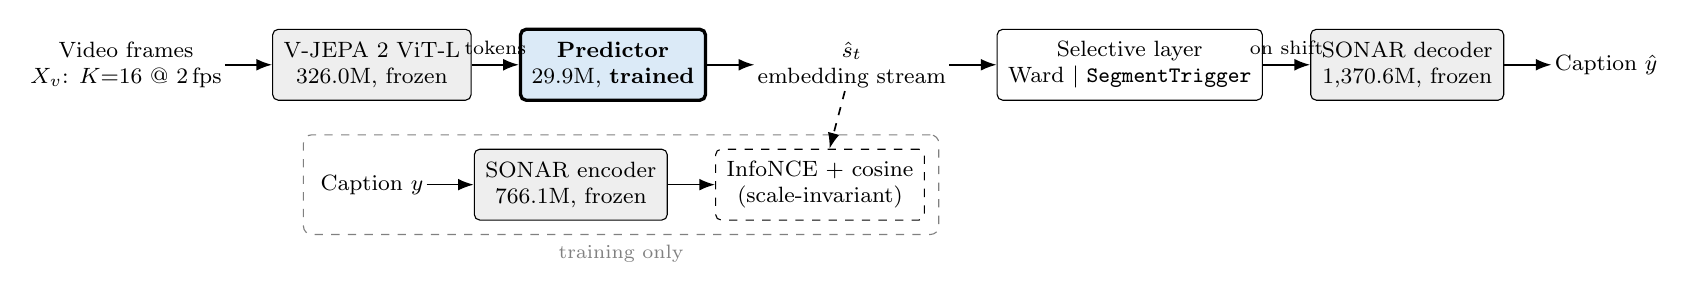
\begin{tikzpicture}[font=\footnotesize, node distance=5mm and 6mm,
  b/.style={draw, rounded corners=2pt, align=center, inner xsep=4pt,
            inner ysep=3pt, minimum height=9mm},
  frozen/.style={b, fill=frz},
  trained/.style={b, fill=hl, very thick},
  io/.style={align=center, inner sep=1pt},
  a/.style={-{Latex[length=2mm]}, semithick}]

  \node[io] (xv) {Video frames\\$X_v$: $K{=}16$ @ 2\,fps};
  \node[frozen, right=of xv] (enc) {V-JEPA~2 ViT-L\\326.0M, frozen};
  \node[trained, right=of enc] (pred) {\textbf{Predictor}\\29.9M, \textbf{trained}};
  \node[io, right=of pred] (shat) {$\hat{s}_t$\\embedding stream};
  \node[b, right=of shat] (sel) {Selective layer\\Ward $\mid$ \texttt{SegmentTrigger}};
  \node[frozen, right=of sel] (dec) {SONAR decoder\\1{,}370.6M, frozen};
  \node[io, right=of dec] (out) {Caption $\hat{y}$};

  \node[io, below=9mm of enc] (y) {Caption $y$};
  \node[frozen, right=of y] (yenc) {SONAR encoder\\766.1M, frozen};
  \node[b, dashed, right=of yenc] (loss) {InfoNCE $+$ cosine\\(scale-invariant)};

  \draw[a] (xv) -- (enc);
  \draw[a] (enc) -- node[above, font=\scriptsize] {tokens} (pred);
  \draw[a] (pred) -- (shat);
  \draw[a] (shat) -- (sel);
  \draw[a] (sel) -- node[above, font=\scriptsize] {on shift} (dec);
  \draw[a] (dec) -- (out);
  \draw[a] (y) -- (yenc);
  \draw[a] (yenc) -- (loss);
  \draw[a, dashed] (shat) -- (loss);

  \begin{scope}[on background layer]
    \node[draw=gray, dashed, rounded corners=3pt, inner sep=5pt,
          fit=(y)(yenc)(loss), label={[gray, font=\scriptsize]below:training only}] {};
  \end{scope}
\end{tikzpicture}}
\caption{LiveJEPA architecture. Only the predictor is trained (tinted); the
2.46B parameters of the two encoders and the decoder stay frozen. At inference the
decoder runs only when the selective layer fires, which is where the saving comes
from. During training the caption is embedded by the SONAR encoder and the
predictor is fitted to that target; at inference that branch is absent.}
\label{fig:arch}
\end{figure*}

\begin{table}[t]
\caption{Pipeline stages. Only the predictor is trained: 1.2\% of the parameters.}
\label{tab:stages}
\centering
\footnotesize
\setlength{\tabcolsep}{4pt}
\begin{tabular}{llrc}
\toprule
stage & component & params & trained \\
\midrule
watch & V-JEPA~2 ViT-L (frozen) & 326.0M & no \\
predict & transformer predictor & 29.9M & \textbf{yes} \\
target space & SONAR text encoder & 766.1M & no \\
speak & SONAR text decoder & 1{,}370.6M & no \\
\bottomrule
\end{tabular}
\end{table}

\subsection{The predictor}
The predictor is a small transformer~\cite{transformer2017} mapping 1024-dimensional
V-JEPA~2 tokens to a 1024-dimensional SONAR embedding, with hidden width 768,
depth 4, 8 heads and dropout 0.1. Training combines an InfoNCE
term~\cite{cpc2018} (temperature 0.07) with a cosine-regression term; both are
scale-invariant, which has a consequence exploited in
Section~\ref{sec:native}. Optimisation uses AdamW~\cite{adamw2019} with learning
rate $3\times10^{-4}$, weight decay 0.05, batch size 32, a 500-step linear warmup
and cosine decay, for 20k steps (30k for the final COIN model).

\subsection{Selective decoding, offline}
Given a stream $S = (s_1,\dots,s_T)$ and a decode budget of $N$ points,
agglomerative Ward-linkage clustering with a temporal-connectivity constraint
partitions $S$ into $N$ contiguous segments; each segment is represented by its
mean embedding, decoded at the segment midpoint. Budget matching is exact: $N$ is
set to the number of points a uniform schedule would spend at the same target
frequency, so the two policies are always compared at equal decoder cost. This
offline policy is what ``adaptive'' denotes in every table below. Fig.~\ref{fig:idea}
shows what the two schedules do differently at an equal budget: uniform spends its
decodes on a clock, adaptive spends them one per semantic plateau.

Two baselines share adaptive's budget. \emph{Uniform} decodes the single stream
step at each fixed-interval point. \emph{Uniform+pool} decodes, at those same
points, the mean of a fixed block of one decode interval, taken from the same
pre-smoothed stream adaptive segments; it differs from adaptive only in where span
boundaries fall, and it is the like-for-like baseline, since VL-JEPA pools under
both schedules. As a reference with no timing at all, one decode per take uses the
mean of the whole stream.

\begin{figure}[t]
\centering
\resizebox{\columnwidth}{!}{%
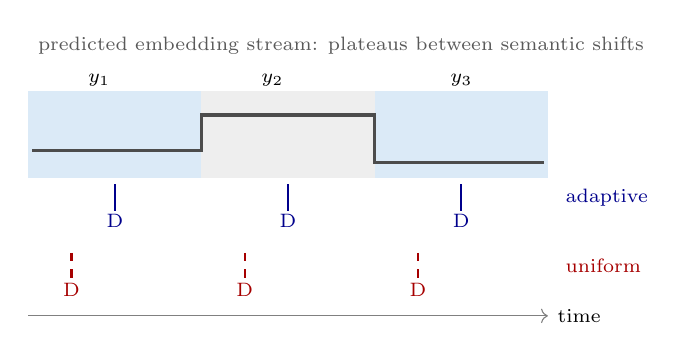
\begin{tikzpicture}[font=\scriptsize, x=1cm, y=1cm]
  % title, clear of everything else
  \node[anchor=south west, gray!70!black] at (0,2.25)
    {predicted embedding stream: plateaus between semantic shifts};

  % segment bands
  \begin{scope}[on background layer]
    \fill[hl] (0,0.8) rectangle (2.2,1.9);
    \fill[frz] (2.2,0.8) rectangle (4.4,1.9);
    \fill[hl] (4.4,0.8) rectangle (6.6,1.9);
  \end{scope}

  % the stream itself: three plateaus with two shifts
  \draw[very thick, gray!60!black]
    (0.05,1.15) -- (2.2,1.15) -- (2.2,1.6) -- (4.4,1.6)
    -- (4.4,1.0) -- (6.55,1.0);

  % annotations, just above the band
  \foreach \x/\l in {0.9/$y_1$, 3.1/$y_2$, 5.5/$y_3$}
    \node[anchor=south, inner sep=1pt] at (\x,1.92) {\l};

  % adaptive: one decode per segment, at its midpoint
  \foreach \x in {1.1,3.3,5.5} {
    \draw[thick, blue!55!black] (\x,0.72) -- (\x,0.38);
    \node[blue!55!black, anchor=north, inner sep=1pt] at (\x,0.38) {D};
  }
  \node[anchor=west, blue!55!black] at (6.7,0.55) {adaptive};

  % uniform: the same number of decodes, on a fixed clock
  \foreach \x in {0.55,2.75,4.95} {
    \draw[thick, dashed, red!65!black] (\x,-0.15) -- (\x,-0.49);
    \node[red!65!black, anchor=north, inner sep=1pt] at (\x,-0.49) {D};
  }
  \node[anchor=west, red!65!black] at (6.7,-0.32) {uniform};

  \draw[->, gray] (0,-0.95) -- (6.6,-0.95) node[right, black] {time};
\end{tikzpicture}}
\caption{Selective decoding at an equal budget. The stream sits on plateaus
between semantic shifts; adaptive places its three decodes one per plateau, at the
midpoint, while uniform places the same three on a fixed clock and can land mid
shift. Quality is scored by matching each annotation $y_i$ to the decode nearest
it in time, so \emph{where} the decodes land is what the metric sees. This is the
clean-stream regime in which placement pays; on a noisy predicted stream,
averaging matters more (Section~\ref{sec:headline}).}
\label{fig:idea}
\end{figure}

\subsection{Pre-smoothing}
Before clustering, the stream may be smoothed with a moving average of window $w$.
The released configuration uses $w=3$; Sections~\ref{sec:coin-pred}
and~\ref{sec:headline} report sweeps and an on/off comparison, since an undisclosed
smoothing setting would otherwise sit under every adaptive number.

\subsection{Selective decoding, online}
A causal trigger cannot see the future. The naive windowed-variance trigger
decodes the mean of the last $W$ embeddings whenever the cosine shift
$1-\cos(s_t, \bar{s}_{t-W:t})$ exceeds $\tau$, but that window straddles the
boundary it has just detected --- mixing old and new meaning --- and timestamps
the decode on the boundary itself. Our \texttt{SegmentTrigger}
(Algorithm~\ref{alg:trigger}) keeps the same detector and changes the emission:
it accumulates the current segment and, when a shift fires, emits the
\emph{previous} segment's mean at that segment's midpoint, accepting one window of
latency. Section~\ref{sec:trigger-results} shows this single change is worth more
than twice the CIDEr of the naive variant.

\begin{algorithm}[t]
\caption{\texttt{SegmentTrigger} (causal, retrospective emission)}
\label{alg:trigger}
\begin{algorithmic}[1]
\STATE \textbf{input:} stream $s_1,s_2,\dots$; window $W$; threshold $\tau$; gap $g$
\STATE $C \leftarrow [\,]$ \COMMENT{current segment}
\FOR{each arriving $s_t$}
  \STATE $\bar{s} \leftarrow \mathrm{mean}(\text{last } W \text{ of } C)$
  \STATE $\delta \leftarrow 1-\cos(s_t,\bar{s})$ \COMMENT{the same detector}
  \IF{$\delta > \tau$ \AND gap since last emission $\geq g$}
    \STATE emit $\mathrm{mean}(C)$ at the \emph{midpoint index} of $C$
    \STATE $C \leftarrow [s_t]$ \COMMENT{start the new segment}
  \ELSE
    \STATE append $s_t$ to $C$
  \ENDIF
\ENDFOR
\STATE emit $\mathrm{mean}(C)$ at its midpoint \COMMENT{flush the final segment}
\end{algorithmic}
\end{algorithm}

\subsection{Native-scale handling}
\label{sec:native}
The SONAR decoder is trained on its encoder's native output scale (mean L2 norm
$\approx$0.196) and returns empty strings for unit-normalised inputs. Because both
predictor losses are scale-invariant, the predictor's raw output norm is
arbitrary. Two consequences are handled throughout: the selective layer clusters
and triggers on \emph{normalised} embeddings, which makes those decisions
scale-free, but pools and returns embeddings at \emph{native} scale for decoding;
and the predictor's output is rescaled to the native norm before it reaches the
decoder. Getting this wrong produces empty captions silently, with no error
anywhere in the pipeline.

\subsection{Implementation and data engine}
Training the predictor at scale required its own engineering. COIN is distributed
as YouTube links, of which a large fraction are dead or throttled, so a three-lane
extraction fleet (a free Kaggle T4, Colab, and a local workstation GPU) worked a
single shared video list with resumable state, fatal-versus-transient error
classification and a streak breaker. It resolved 8{,}984 of 9{,}023 training
videos (99.6\%; 1{,}650 links were permanently dead) into a 26{,}360-clip feature
cache of V-JEPA~2 tokens paired with SONAR targets. Evaluation splits are
video-level and stratified by class, so no evaluation video is seen in training,
and cached streams are keyed by checkpoint so that a rerun never mixes
checkpoints. The complete pipeline also runs as a browser application that streams
captions from uploaded video or a webcam and displays the trigger's own signal
against $\tau$, which is how the mechanism was demonstrated interactively.

\section{Experimental Setup}

\subsection{Datasets}
Table~\ref{tab:data} summarises the three corpora. COIN~\cite{coin2019} supplies
instructional video with time-stamped step labels, used both for predictor
training and for evaluation. EgoExo4D~\cite{egoexo4d2024} supplies two annotation
granularities over the same videos: \emph{keysteps}, which are coarse and
temporally stable, and \emph{atomic action descriptions}, which are dense at
roughly one event every two seconds and are the benchmark VL-JEPA reports on. For
the atomic protocol we select the 218 validation takes whose annotation counts
are closest to the paper's $\approx$143 per video, and a 40-take subset of those
for the predicted-stream experiments, which cost about 23 minutes of encoding per
take. Action100M~\cite{action100m2026}, generated over
HowTo100M~\cite{howto100m2019} videos, supplies one training rung through its
10\% preview release.

\begin{table}[t]
\caption{Corpora and how they are used. Density is annotations per unit time.}
\label{tab:data}
\centering
\footnotesize
\setlength{\tabcolsep}{3pt}
\begin{tabular}{llll}
\toprule
corpus & granularity & density & role \\
\midrule
COIN & step labels & $\approx$1 / 5~s & train + eval \\
EgoExo4D & keysteps & $\approx$1 / 15~s & mechanism \\
EgoExo4D & atomic descr. & $\approx$1 / 2~s & paper's benchmark \\
Action100M & action descr. & --- & controlled rung \\
\bottomrule
\end{tabular}
\end{table}

\subsection{Metrics}
Following the original protocol, each ground-truth annotation $(t_i, y_i)$ is
matched to the nearest decoded caption in time, and CIDEr-D~\cite{cider2015} is
computed over those aligned pairs:
\begin{equation}
j(i) = \arg\min_{j} \lvert t_i - \hat{t}_j \rvert, \qquad
\text{CIDEr-D}\big(\{(y_i, \hat{y}_{j(i)})\}_i\big),
\end{equation}
where $(\hat{t}_j, \hat{y}_j)$ are the decoded timepoints and captions. This
rewards saying the right thing at the right time and penalises both wrong captions
and captions at the wrong moment.

CIDEr counts n-grams, so a semantically correct caption in a different register
scores near zero --- a failure we hit directly in Section~\ref{sec:headline}. We
therefore also report a time-aligned \emph{semantic} metric that keeps the same
alignment but scores in embedding space:
\begin{equation}
\mathrm{SEM} = \frac{1}{n}\sum_{i=1}^{n}
\cos\big(e_{j(i)},\; \mathrm{SONAR}(y_i)\big),
\end{equation}
where $e_{j(i)}$ is the embedding actually selected for decoding at the matched
point (for adaptive, the pooled segment mean). It needs no text generation, which
also makes it cheap enough to run controls against.

\subsection{Protocol, hardware and statistics}
Each experiment sweeps a target decoding frequency from 1.0~Hz down to 0.01~Hz,
with adaptive budget-matched to uniform at every point. Evaluations run in two
modes: \texttt{gt}, where the stream is built from ground-truth captions and so
isolates the selective mechanism, and \texttt{predictor}, the full
video-to-caption system. A local NVIDIA T1000 (8~GB) runs inference, evaluation
and most training; a free Kaggle T4 ran the first wide retrain and, with Colab,
the feature extraction; one rented RTX~4090 trained the Action100M rung. Where
per-take scores exist, methods are compared with a paired bootstrap over
takes~\cite{efron1993}, 5{,}000 resamples, 95\% intervals; pairing is the correct
design because both methods see the identical take, so take-difficulty variance
cancels.

\section{Results}
\label{sec:results}

\subsection{The mechanism on ground-truth streams}
On clean streams built from ground-truth captions, adaptive decoding beats uniform
across the mid-band of decode rates (Table~\ref{tab:gt}, Figs.~\ref{fig:coin-gt}
and~\ref{fig:keystep}). On COIN, adaptive holds CIDEr~$\approx$7.7 at 0.20~Hz,
which uniform reaches only near 0.31~Hz --- $\approx 1.6\times$ fewer decoder
calls at equal quality. On EgoExo4D keysteps it holds the 8.20 plateau down to
0.20~Hz where uniform needs 0.50~Hz, i.e. $\approx 2.5\times$.

Two honest qualifications follow from the full sweep, which is why we print every
budget. At 1~Hz the two policies coincide, because the budget then covers the
whole stream. Below 0.10~Hz the ordering reverses on both streams: with only a
handful of decodes per video, uniform's even spacing covers the timeline better
than a few segment means, and adaptive also spends marginally fewer decodes there
(187 against 201 at 0.05~Hz on COIN). This is mid-band dominance, not the
full-range Pareto dominance the original paper reports over 0.01--2~Hz.

\begin{table}[t]
\caption{Ground-truth streams: time-aligned CIDEr-D. COIN validation (26 videos)
and EgoExo4D keysteps (10 takes). Bold marks the winner at each budget.}
\label{tab:gt}
\centering
\footnotesize
\setlength{\tabcolsep}{5pt}
\begin{tabular}{rcccc}
\toprule
& \multicolumn{2}{c}{COIN steps} & \multicolumn{2}{c}{EgoExo4D keysteps} \\
\cmidrule(lr){2-3}\cmidrule(lr){4-5}
Hz & uniform & adaptive & uniform & adaptive \\
\midrule
1.00 & 8.81 & 8.81 & --- & --- \\
0.50 & 8.47 & \textbf{8.79} & 8.20 & 8.20 \\
0.35 & 7.92 & \textbf{8.67} & 8.12 & \textbf{8.20} \\
0.20 & 6.83 & \textbf{7.72} & 7.75 & \textbf{8.20} \\
0.10 & 4.94 & \textbf{5.27} & 6.54 & \textbf{7.38} \\
0.05 & \textbf{3.77} & 3.53 & \textbf{4.70} & 4.16 \\
0.02 & \textbf{3.54} & 2.29 & \textbf{2.37} & 1.58 \\
0.01 & \textbf{3.46} & 2.04 & \textbf{1.49} & 0.74 \\
\bottomrule
\end{tabular}
\end{table}

\begin{figure}[t]
\centering
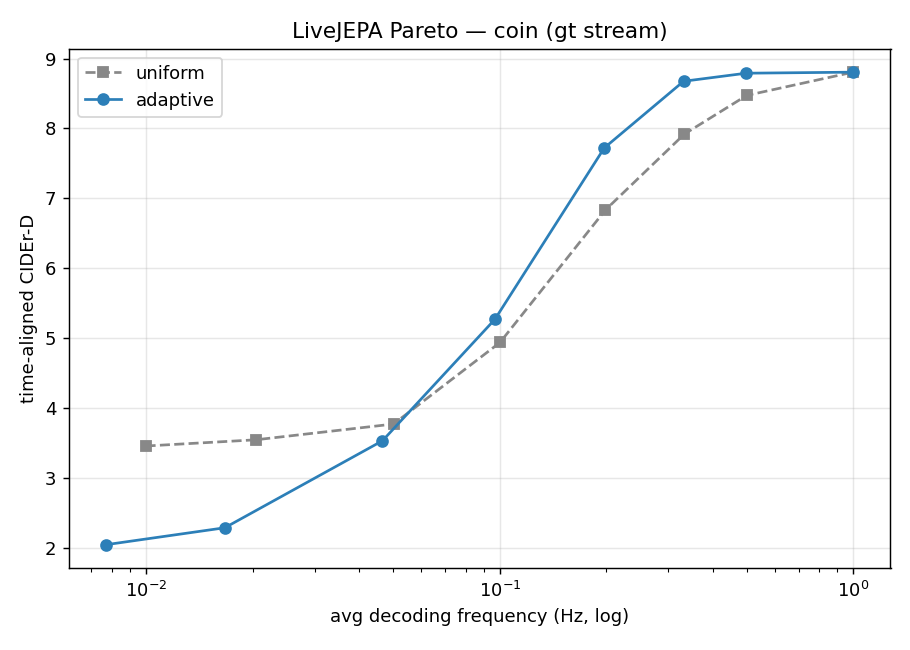
\includegraphics[width=\columnwidth]{figures/results_coin_gt.png}
\caption{COIN validation, ground-truth stream (26 videos). Adaptive holds
CIDEr~$\approx$7.7 at 0.20~Hz, a rate uniform does not reach until
$\approx$0.31~Hz. Below 0.10~Hz uniform recovers.}
\label{fig:coin-gt}
\end{figure}

\begin{figure}[t]
\centering
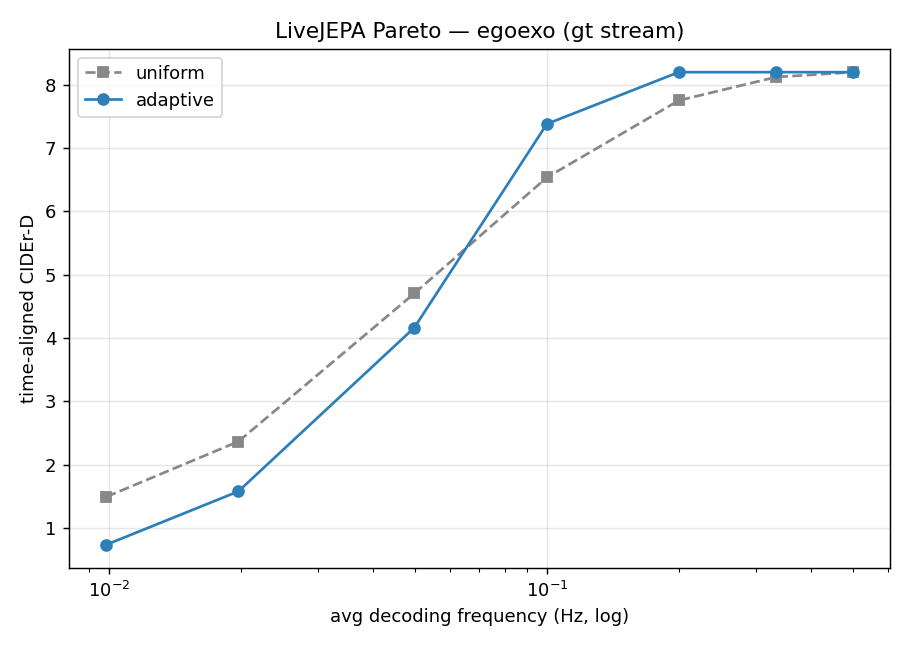
\includegraphics[width=\columnwidth]{figures/results_egoexo_keystep.png}
\caption{EgoExo4D keysteps, ground-truth stream (10 takes). Adaptive holds the
8.20 plateau down to 0.20~Hz against uniform's 0.50~Hz, with the same low-rate
crossover.}
\label{fig:keystep}
\end{figure}

\subsection{The online trigger correction}
\label{sec:trigger-results}
A streaming system cannot use the offline segmenter, so the causal trigger decides
whether the mechanism is deployable at all. Table~\ref{tab:ablation} and
Fig.~\ref{fig:ablation} compare the four policies on the ablation harness (the first 240~s of 6 keystep takes, with a
small jitter added to the ground-truth stream, which is why absolute values differ
from Table~\ref{tab:gt}). The naive windowed-variance trigger reaches only
$\approx$3.5 CIDEr, far below uniform at the same rate; the corrected
\texttt{SegmentTrigger} reaches 7.24--7.72, recovering the offline Ward result
(6.72) and edging past it. The gain comes entirely from \emph{when} the segment is
emitted, since the detector is identical.

\begin{table}[t]
\caption{Method ablation at $\approx$0.1~Hz (6 keystep takes, first 240~s).
Online methods cannot be budget-matched exactly, so their realised rate is shown.}
\label{tab:ablation}
\centering
\footnotesize
\setlength{\tabcolsep}{5pt}
\begin{tabular}{lcc}
\toprule
policy & avg Hz & CIDEr \\
\midrule
uniform & 0.100 & 6.06 \\
adaptive, offline Ward & 0.100 & 6.72 \\
online, naive variance trigger & 0.103 & 3.54 \\
\textbf{online, \texttt{SegmentTrigger}} & 0.103 & \textbf{7.72} \\
\bottomrule
\end{tabular}
\end{table}

The naive trigger's weakness is not a badly chosen threshold.
Table~\ref{tab:grid} sweeps its window $W$ and threshold $\tau$: CIDEr is almost
flat in $\tau$, degrades sharply at $W=16$, and never approaches the corrected
variant at any setting. Two further ablations on the same harness: mean-pooling a
segment beats decoding its exact midpoint embedding at the denser rates (7.97
against 7.80 at 0.35~Hz; 7.95 against 7.77 at 0.20~Hz) and loses slightly at
0.10~Hz (6.72 against 6.94), and pre-smoothing the ground-truth stream hurts
monotonically at 0.20~Hz (7.95, 7.55 and 7.50 for $w=1,3,5$), because at keystep
granularity it blurs boundaries that are already crisp.

\begin{table}[t]
\caption{Sensitivity of the \emph{naive} online trigger to its window $W$ and
threshold $\tau$ (CIDEr; 6 keystep takes). No setting approaches the corrected
trigger's 7.2--7.7.}
\label{tab:grid}
\centering
\footnotesize
\setlength{\tabcolsep}{6pt}
\begin{tabular}{lccc}
\toprule
& $\tau=0.10$ & $\tau=0.15$ & $\tau=0.20$ \\
\midrule
$W=4$ & 3.42 & 3.45 & 3.43 \\
$W=8$ & 3.79 & 3.68 & 3.64 \\
$W=16$ & 2.49 & 2.14 & 2.18 \\
\bottomrule
\end{tabular}
\end{table}

\begin{figure}[t]
\centering
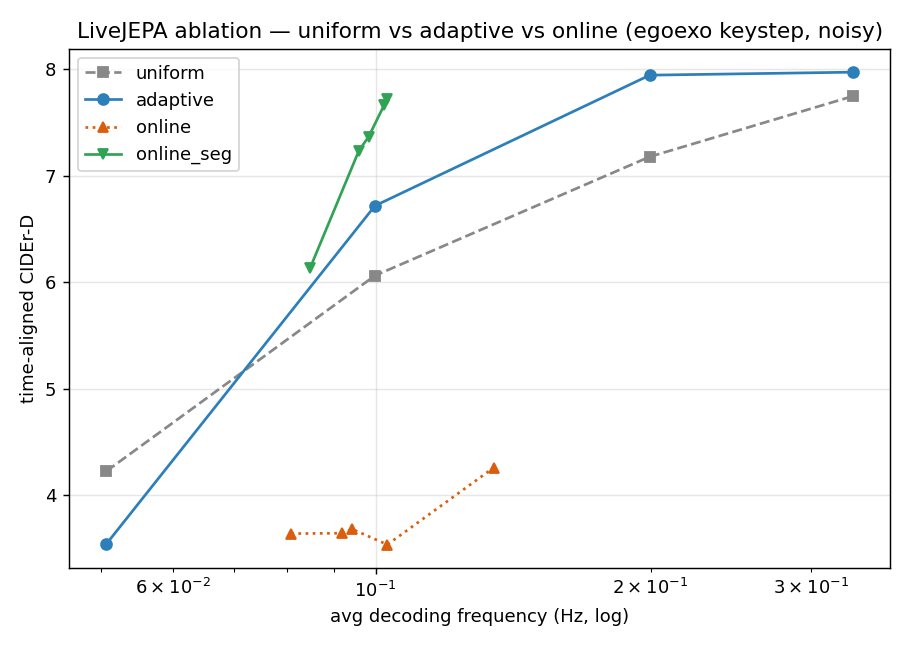
\includegraphics[width=\columnwidth]{figures/results_ablation_methods.png}
\caption{Method ablation at $\approx$0.10~Hz on EgoExo4D keysteps. The corrected
trigger recovers the offline result and edges past it, which is what makes the
causal path viable.}
\label{fig:ablation}
\end{figure}

\subsection{The full predicted pipeline on COIN}
\label{sec:coin-pred}
Replacing the ground-truth stream with the system's own predictions changes the
picture. Table~\ref{tab:coin-pred} reports the full pipeline on 7 held-out COIN
videos. Two things stand out. Absolute CIDEr is 2.6--3.0, against $\leq$1.2 for an
earlier narrower predictor, so predictor quality --- not the selective layer ---
drives absolute quality. And adaptive no longer dominates cleanly: it wins at high
(1.0, 0.5~Hz) and sparse (0.1~Hz) rates, while uniform peaks at 0.20~Hz and takes
the mid-band.

\begin{table}[t]
\caption{Predictor-in-the-loop Pareto, 7 held-out COIN validation videos
(2{,}962-clip predictor, no pre-smoothing).}
\label{tab:coin-pred}
\centering
\footnotesize
\setlength{\tabcolsep}{6pt}
\begin{tabular}{rccl}
\toprule
Hz & uniform & adaptive & winner \\
\midrule
1.00 & 2.611 & \textbf{2.814} & adaptive \\
0.50 & 2.644 & \textbf{2.779} & adaptive \\
0.35 & \textbf{2.856} & 2.735 & uniform \\
0.20 & \textbf{2.960} & 2.411 & uniform \\
0.10 & 2.124 & \textbf{2.415} & adaptive \\
0.05 & 2.191 & 2.150 & $\approx$tie \\
0.02 & 1.668 & 1.645 & $\approx$tie \\
0.01 & \textbf{1.960} & 0.977 & uniform \\
\bottomrule
\end{tabular}
\end{table}

Is the mid-band loss a tuning artifact? Table~\ref{tab:tuning} says no. Sweeping
the pre-smoothing window against the linkage criterion on cached streams --- with
the identical decoder and metric, and with the un-smoothed Ward cell reproducing
Table~\ref{tab:coin-pred} to three decimals as a self-check --- every configuration
is worse than uniform on average, and at 0.20~Hz uniform beats all eight. The
attenuation is a property of predictor-stream noise, not of a mis-set threshold.
Average linkage is uniformly worse than Ward, and smoothing never helps on this
stream, although the released configuration keeps $w=3$, which slightly understates
adaptive here.

\begin{table}[t]
\caption{Trigger-tuning sweep on the predicted COIN stream: wins over uniform out
of four mid-band budgets, and mean CIDEr difference. The un-smoothed Ward baseline
is the best of the eight.}
\label{tab:tuning}
\centering
\footnotesize
\setlength{\tabcolsep}{6pt}
\begin{tabular}{lcc}
\toprule
configuration & wins / 4 & mean $\Delta$ vs uniform \\
\midrule
\textbf{$w=1$, ward} & \textbf{2 / 4} & \textbf{$-0.061$} \\
$w=3$, ward & 1 / 4 & $-0.199$ \\
$w=7$, ward & 1 / 4 & $-0.211$ \\
$w=5$, ward & 1 / 4 & $-0.262$ \\
$w=1$, average & 0 / 4 & $-0.269$ \\
$w=3$, average & 0 / 4 & $-0.421$ \\
$w=7$, average & 0 / 4 & $-0.542$ \\
$w=5$, average & 0 / 4 & $-0.564$ \\
\bottomrule
\end{tabular}
\end{table}

\subsection{Data, not architecture, is the binding constraint}
Since predictor quality limits the full-system result, we scaled training data
while holding architecture, loss and both validation sets fixed
(Table~\ref{tab:scaling}). Accuracy rose $+0.113$ cosine over the last
$4.8\times$ of data without saturating. Because the last rung also trained longer,
we report its 20k-step checkpoint too: $+0.099$ of the gain is present at matched
training length, so it is data rather than the extra steps. Predictions grew
\emph{more} diverse as data grew (pred--pred cosine $0.527 \rightarrow 0.408$),
which excludes representation collapse. The smaller frozen validation set
saturates earlier, adding nothing at matched length --- a reminder that a small
benchmark stops measuring progress before a large one does.

\begin{table}[t]
\caption{Data scaling at fixed architecture: cosine to the SONAR target on a
frozen 137-sample and a diverse 956-sample validation set, and mean pairwise
cosine between predictions (lower is more diverse).}
\label{tab:scaling}
\centering
\footnotesize
\setlength{\tabcolsep}{6pt}
\begin{tabular}{rrccc}
\toprule
clips & steps & 137-val & 956-val & pred--pred \\
\midrule
2{,}962 & 20k & 0.772 & 0.667 & 0.527 \\
5{,}529 & 20k & 0.883 & 0.733 & 0.467 \\
26{,}360 & 20k & 0.882 & 0.832 & 0.394 \\
\textbf{26{,}360} & \textbf{30k} & \textbf{0.897} & \textbf{0.846} & \textbf{0.408} \\
\bottomrule
\end{tabular}
\end{table}

Does a better predictor change the regime? Fig.~\ref{fig:scaling} repeats the
full-system evaluation with the weakest and the strongest checkpoint on the same
7 videos. Absolute CIDEr roughly doubles (4.9--5.4 against 2.4--3.0 in the
0.2--1.0~Hz band), yet the shape is unchanged: adaptive wins at 1.0 and 0.1~Hz,
uniform holds 0.2--0.5~Hz, coming closest at 0.35~Hz (5.07 against 5.04). The
mid-band advantage of uniform is therefore not an artifact of a weak predictor; it
tracks COIN's intrinsic step cadence of roughly one event per five seconds, where
even spacing is close to optimal by construction.

\begin{figure*}[t]
\centering
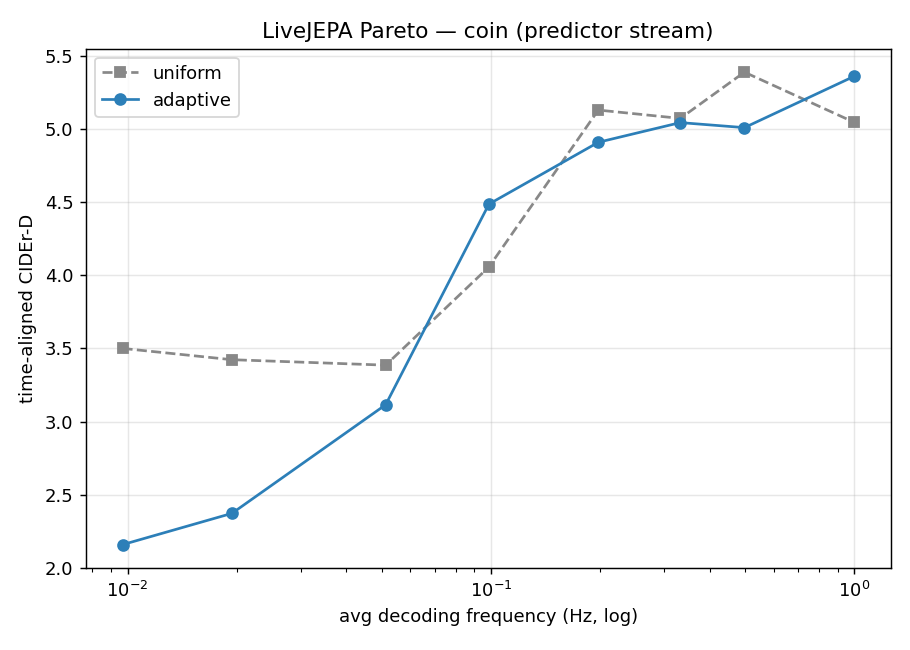
\includegraphics[width=0.48\textwidth]{figures/results_coin_predictor_c1final.png}
\hfill
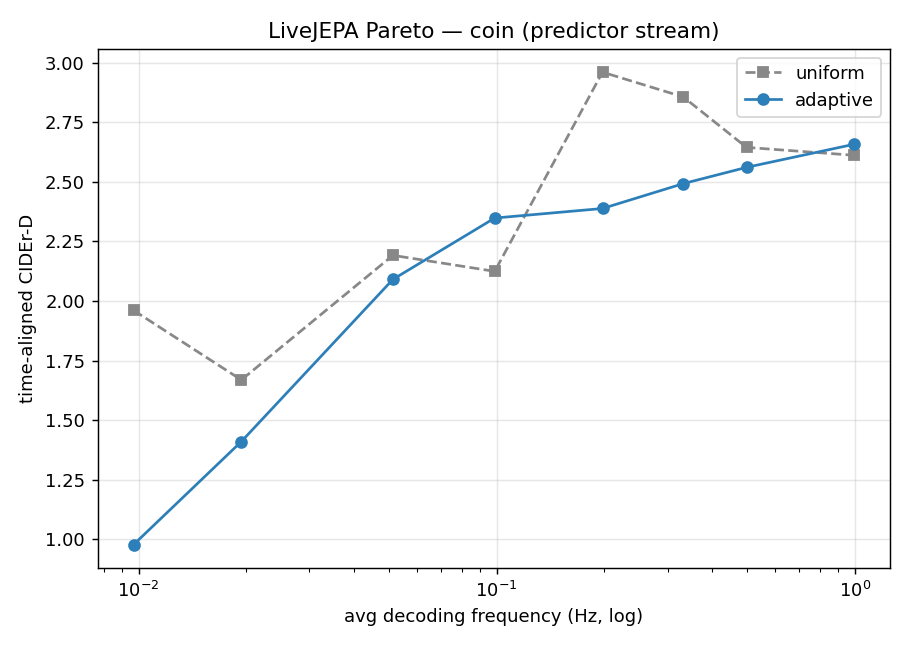
\includegraphics[width=0.48\textwidth]{figures/results_coin_predictor_c1old.png}
\caption{Identical protocol, two predictors on the same 7 held-out COIN videos:
the final 26{,}360-clip checkpoint (left) and the earlier 2{,}962-clip one
(right), which score cosine 0.846 and 0.667 on the same validation set. The
absolute lift comes from training data; the regime pattern does not move.}
\label{fig:scaling}
\end{figure*}

\subsection{Training on the paper's own corpus}
\label{sec:a100m}
VL-JEPA trains on Action100M, we trained on COIN step labels, and the obvious
objection is that the difference explains everything. Table~\ref{tab:a100m} tests
it directly. Extraction throttling capped the Action100M rung at 6{,}710 training
clips, which fortuitously makes it a near-exact scale match to the 5{,}529-clip
COIN rung rather than a scale-up. Both COIN-trained models beat the
Action100M-trained model \emph{on Action100M's own validation set}, and the
scale-matched pair is decisive: C1-mid saw fewer clips for the same 20k steps yet
scores 0.401 against 0.348.

\begin{table}[t]
\caption{Predictor cosine on three validation sets. C1-mid against C2 is the
scale-matched control; C3 adds Action100M to COIN rather than replacing it.}
\label{tab:a100m}
\centering
\footnotesize
\setlength{\tabcolsep}{3pt}
\begin{tabular}{lccc}
\toprule
model (data, steps) & COIN-137 & COIN-956 & A100M-160 \\
\midrule
C1-final (26{,}360 COIN, 30k) & \textbf{0.897} & \textbf{0.846} & 0.386 \\
C1-mid (5{,}529 COIN, 20k) & 0.883 & 0.733 & \textbf{0.401} \\
C2 (6{,}710 A100M, 20k) & 0.359 & 0.392 & 0.348 \\
C3 (33{,}573 combined, 30k) & 0.875 & 0.824 & 0.390 \\
\bottomrule
\end{tabular}
\end{table}

Our first explanation was label noise. Measurement contradicted it.
Table~\ref{tab:vocab} shows the corpora differ mainly in target-vocabulary
entropy: COIN is effectively closed-set, with 747 recurring step labels each seen
about 36 times, while the Action100M preview is genuinely open-vocabulary, with
nearly every caption unique. Inspection confirms its captions are sensible actions
rather than noise. The decoded outputs match the entropy account: with roughly one
example per target, C2 acquired the \emph{distribution of phrasings} without
binding phrasing to content, while the COIN models' closed vocabulary transfers
out of domain as a coarse but useful prior. Adding Action100M as augmentation (C3)
does not rescue it either: both COIN scores drop by 0.022 and exact matches on the
frozen benchmark fall from 7/10 to 5/10, with open-vocabulary targets contaminating
previously exact closed-set outputs. Table~\ref{tab:qual} gives representative
examples.

\begin{table}[t]
\caption{Target-vocabulary statistics of the two training corpora.}
\label{tab:vocab}
\centering
\footnotesize
\setlength{\tabcolsep}{6pt}
\begin{tabular}{lrrr}
\toprule
corpus & clips & unique captions & repeats / caption \\
\midrule
COIN & 26{,}863 & 747 (3\%) & \textbf{36.0} \\
Action100M & 6{,}710 & 6{,}096 (91\%) & \textbf{1.1} \\
\bottomrule
\end{tabular}
\end{table}

\begin{table}[t]
\caption{Representative decoded outputs. The failure modes differ by corpus: fuzzy
object detail (COIN), register mismatch (cross-domain), unbound phrasing (open
vocabulary), and contamination when the two are mixed.}
\label{tab:qual}
\centering
\footnotesize
\setlength{\tabcolsep}{3pt}
\begin{tabular}{p{0.44\columnwidth}p{0.44\columnwidth}}
\toprule
target & decoded \\
\midrule
``open the car key cover'' & ``open the back lid'' \\
``stand up with straight legs'' & exact match \\
``the camera wearer takes a tire lever from the table'' & ``remove the chain'' \\
``Get a needle'' (A100M) & ``Push the squeeze of the treats.'' \\
``squat and hold the barbell'' (C3) & ``sitbar and hold the barbell'' \\
\bottomrule
\end{tabular}
\end{table}

This also qualifies our own scaling result: it is measured on a 747-label closed
set, so part of what improves is closed-set discrimination rather than open-ended
captioning, and cosine scores across the two corpora are not commensurable. The
defensible claim is narrow: open-vocabulary supervision needs orders of magnitude
more data than closed-set supervision to reach comparable predictive accuracy, so
a low-resource reconstruction is better served by a small closed-vocabulary corpus.

\subsection{The boundary: atomic descriptions}
\label{sec:boundary}
We then ran the paper's benchmark with a \emph{ground-truth} stream, on the 218
density-matched validation takes (Table~\ref{tab:atomic},
Fig.~\ref{fig:atomic}). Uniform wins at every frequency. At roughly one event
every two seconds the stream is saturated with change and offers nothing for a
segmenter to exploit, so budget-matched segment means can only blur what uniform
samples directly.

Far from contradicting the mechanism, this completes the picture from the
ground-truth experiments: keysteps at $\approx$1 event / 15~s are redundant and
adaptive wins $\approx 2.5\times$; atomic annotations at $\approx$1 event / 2~s are
saturated and adaptive loses everywhere. The benefit tracks redundancy
monotonically. It also sharpens the question, because the paper's positive result
on this benchmark came from its \emph{predicted} stream, not from annotations.

\begin{table}[t]
\caption{EgoExo4D atomic descriptions, 218 density-matched validation takes,
ground-truth stream. Uniform wins at every frequency.}
\label{tab:atomic}
\centering
\footnotesize
\setlength{\tabcolsep}{8pt}
\begin{tabular}{rcc}
\toprule
Hz & uniform & adaptive \\
\midrule
1.00 & \textbf{4.48} & 3.57 \\
0.50 & \textbf{3.47} & 3.11 \\
0.35 & \textbf{2.91} & 2.79 \\
0.20 & \textbf{2.31} & 2.26 \\
0.10 & \textbf{1.78} & 1.60 \\
0.05 & \textbf{1.40} & 1.21 \\
0.02 & \textbf{1.08} & 0.89 \\
0.01 & \textbf{0.91} & 0.76 \\
\bottomrule
\end{tabular}
\end{table}

\begin{figure}[t]
\centering
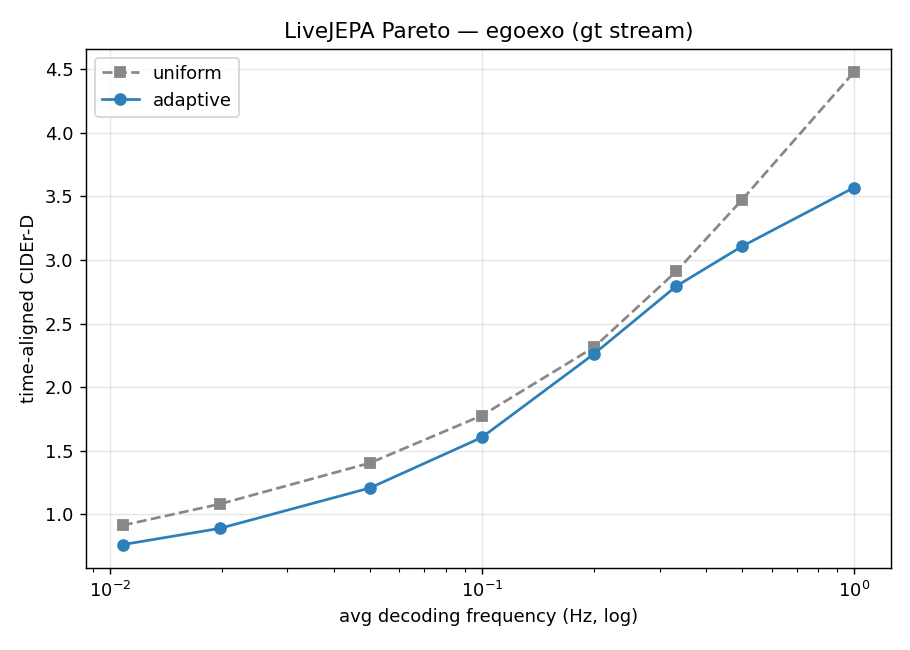
\includegraphics[width=\columnwidth]{figures/results_egoexo_atomic_218.png}
\caption{The redundancy boundary: on raw atomic annotations, uniform wins at every
frequency. Fig.~\ref{fig:headline} shows the same benchmark on the predicted
stream.}
\label{fig:atomic}
\end{figure}

\subsection{The predicted stream: averaging, not placement}
\label{sec:headline}
Testing the predicted stream required a predictor that speaks EgoExo. Our
COIN-trained model was semantically reasonable but stylistically alien --- it
emits imperatives such as ``remove the chain'' where annotations read ``the camera
wearer takes a tire lever from the table with his right hand'' --- which floored
CIDEr at 0.012 for \emph{both} methods: an unmeasurable comparison rather than a
result. We therefore trained an in-domain predictor on 11{,}556 (window, caption)
pairs from 627 EgoExo validation takes for 20k steps, excluding the 40 evaluation
takes and holding out 25 more for gating (cosine 0.599, pred--pred 0.325).

Adaptive decodes the mean of each segment of a pre-smoothed stream, whereas plain
uniform decodes a single stream step. VL-JEPA pools under both schedules, so we
score uniform+pool (Section~\ref{sec:method}) beside them at every budget, and one
decode per take as a reference with no timing at all (Table~\ref{tab:headline},
Fig.~\ref{fig:headline}).

Against plain uniform, adaptive wins 7 of 8 budgets, losing only the degenerate
0.011~Hz point of about two decodes per take, and absolute quality rises $25\times$
from training in-domain. Plain uniform's CIDEr barely depends on rate here --- it
stays between 0.278 and 0.310 at every budget except 0.02~Hz --- and, anchored on
its best score at any rate (0.310 at 3{,}537 decodes), adaptive matches it at
0.050~Hz with 357 decodes: $\approx 9.9\times$ fewer decoder invocations.

That comparison, however, confounds placement with averaging. Pooling alone lifts
uniform above its single-point version at every budget, by 5--26\%, and once
pooling is matched the advantage disappears: uniform+pool scores higher than
adaptive at six of eight budgets, and its best score (0.358 at 2{,}357 decodes)
exceeds adaptive's best anywhere (0.348), so no efficiency multiple can be quoted
against it. A single caption per take --- the mean of its whole stream, 40 decodes
for the whole set --- scores 0.284, about what plain uniform reaches with 1{,}412
decodes. EgoExo takes are repetitive enough (mean pairwise caption similarity
0.669) that a representative caption matches many annotations wherever it is
placed, which bounds how much any placement policy can show on this protocol.

\begin{table}[t]
\caption{Headline: EgoExo4D atomic descriptions, 40 held-out takes, predicted
stream from the in-domain predictor. Time-aligned CIDEr-D; the best schedule at
each budget is tinted. One decode per take scores 0.284.}
\label{tab:headline}
\centering
\footnotesize
\setlength{\tabcolsep}{5pt}
\begin{tabular}{rrccc}
\toprule
avg Hz & decodes & uniform & adaptive & uniform+pool \\
\midrule
0.998 & 7072 & 0.296 & 0.330 & \best{0.335} \\
0.499 & 3537 & 0.310 & \best{0.348} & 0.342 \\
0.333 & 2357 & 0.299 & 0.340 & \best{0.358} \\
0.199 & 1412 & 0.287 & 0.333 & \best{0.341} \\
0.100 & 706 & 0.282 & 0.331 & \best{0.338} \\
0.050 & 357 & 0.278 & \best{0.338} & 0.319 \\
0.020 & 140 & 0.249 & 0.312 & \best{0.314} \\
0.011 & 76 & 0.305 & 0.302 & \best{0.322} \\
\bottomrule
\end{tabular}
\end{table}

\begin{figure}[t]
\centering
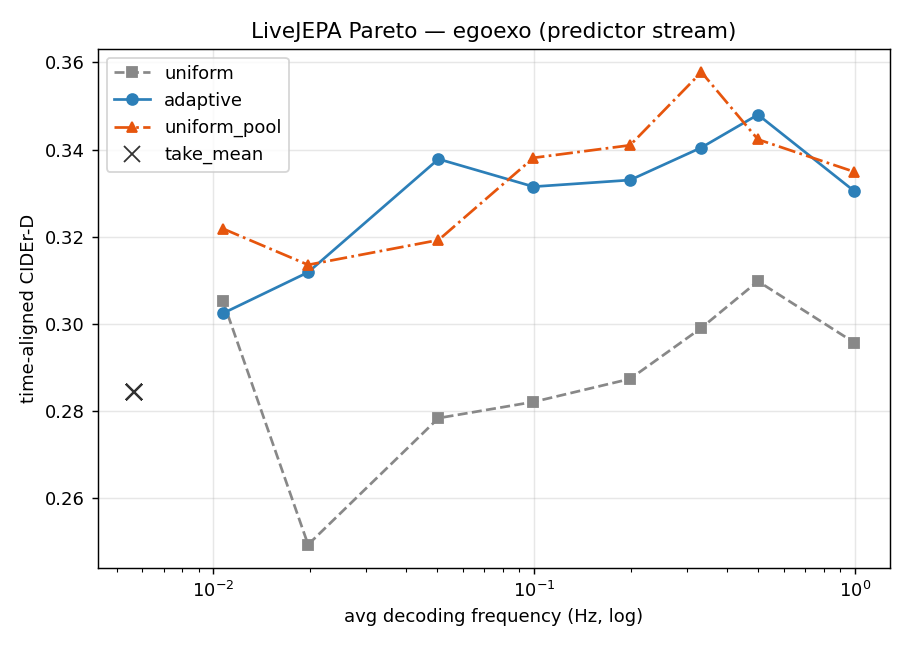
\includegraphics[width=\columnwidth]{figures/results_egoexo_predictor_40_indomain_pooled.png}
\caption{Headline result. The atomic-description benchmark of
Fig.~\ref{fig:atomic}, on 40 of its takes, with the stream predicted. Adaptive
beats single-point uniform at 7 of 8 budgets, but uniform with the same pooling
matches it; the cross is one decode per take.}
\label{fig:headline}
\end{figure}

\subsection{Controls, and what they missed}
An earlier out-of-domain attempt appeared to show adaptive winning on the semantic
metric, and its controls revealed the effect was denoising rather than selection
(Fig.~\ref{fig:rejected}). We repeated those controls in domain and added two.
Every one of them compared adaptive with an \emph{unpooled} baseline, which is why
none caught the confound above.

\emph{Does the metric see timing at all?} Its mean lift over a shuffled alignment
rises from $+0.0012$ out-of-domain --- effectively blind --- to $+0.0225$--$0.0284$
in-domain. This finding stands: the metric does register timing.

\emph{Is the gain just averaging?} With mean-pooling disabled, adaptive kept a flat
$+0.031$--$0.040$ advantage over uniform at every frequency, which we first read as
temporal selection. But disabling pooling left the 3-step pre-smoothing on the
adaptive stream alone, so each ``exact'' adaptive point was still a three-step
average. Given the same smoothing, uniform points score within 0.003 of adaptive's
at every budget (Fig.~\ref{fig:controls}): the flat margin was the smoothing. With
no smoothing on either side, adaptive trails uniform+pool on the semantic metric at
all eight budgets, by 0.009--0.016.

\emph{Is it just spreading decodes out?} Adaptive beats random placement at the
same budget at 8 of 8 budgets, while uniform is indistinguishable from random
(0.597 against 0.596 averaged over budgets). The random points were unpooled too,
however, so this control also measured averaging.

\emph{Is it the smoothing?} Against plain uniform, no (Table~\ref{tab:robust}).
With the pre-smoothing disabled, adaptive wins the same seven budgets, the cell
behind the $9.9\times$ figure is unchanged (0.3379 against 0.3378), and only the
two highest rates narrow, from $\approx+0.035$ to $\approx+0.010$.

\begin{table}[t]
\caption{Robustness of the comparison with plain uniform to pre-smoothing: CIDEr
with the released $w=3$ and with smoothing disabled ($w=1$). The winners are
identical.}
\label{tab:robust}
\centering
\footnotesize
\setlength{\tabcolsep}{5pt}
\begin{tabular}{rccc}
\toprule
Hz & uniform & adaptive $w{=}3$ & adaptive $w{=}1$ \\
\midrule
1.000 & 0.296 & \textbf{0.330} & 0.307 \\
0.500 & 0.310 & \textbf{0.348} & 0.320 \\
0.350 & 0.299 & \textbf{0.340} & 0.340 \\
0.200 & 0.287 & 0.333 & \textbf{0.341} \\
0.100 & 0.282 & 0.331 & \textbf{0.336} \\
0.050 & 0.278 & 0.338 & \textbf{0.338} \\
0.020 & 0.249 & \textbf{0.312} & 0.309 \\
0.011 & \textbf{0.305} & 0.302 & 0.297 \\
\bottomrule
\end{tabular}
\end{table}

\begin{figure*}[t]
\centering
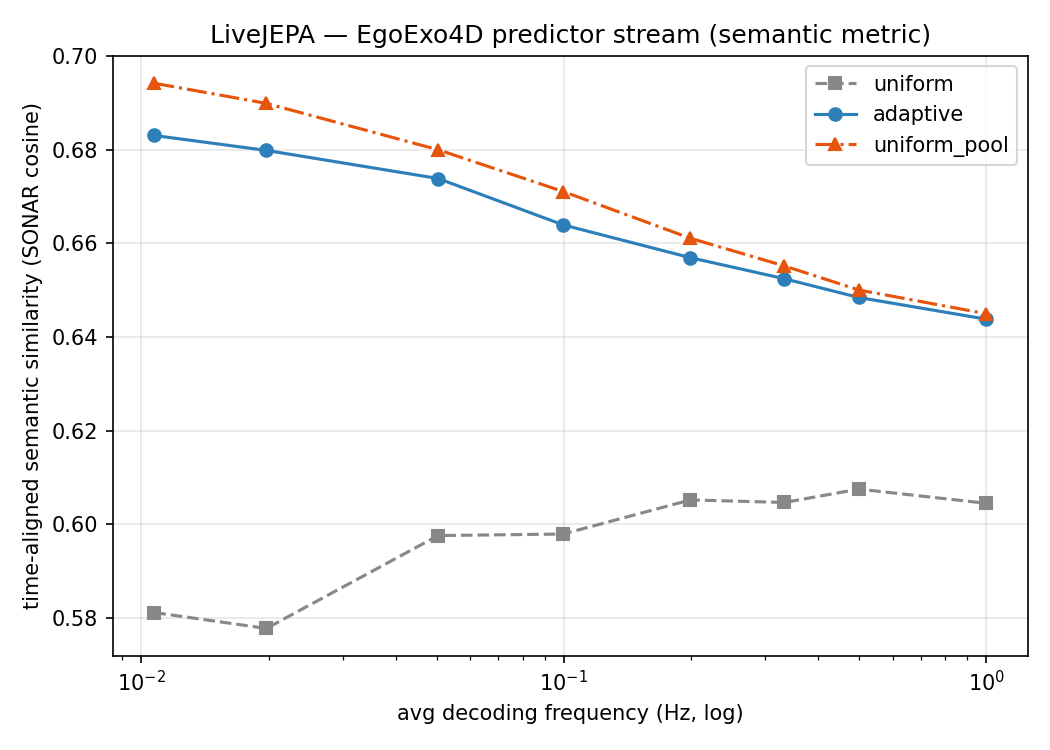
\includegraphics[width=0.48\textwidth]{figures/results_egoexo_predictor_40_indomain_semantic_pooled.png}
\hfill
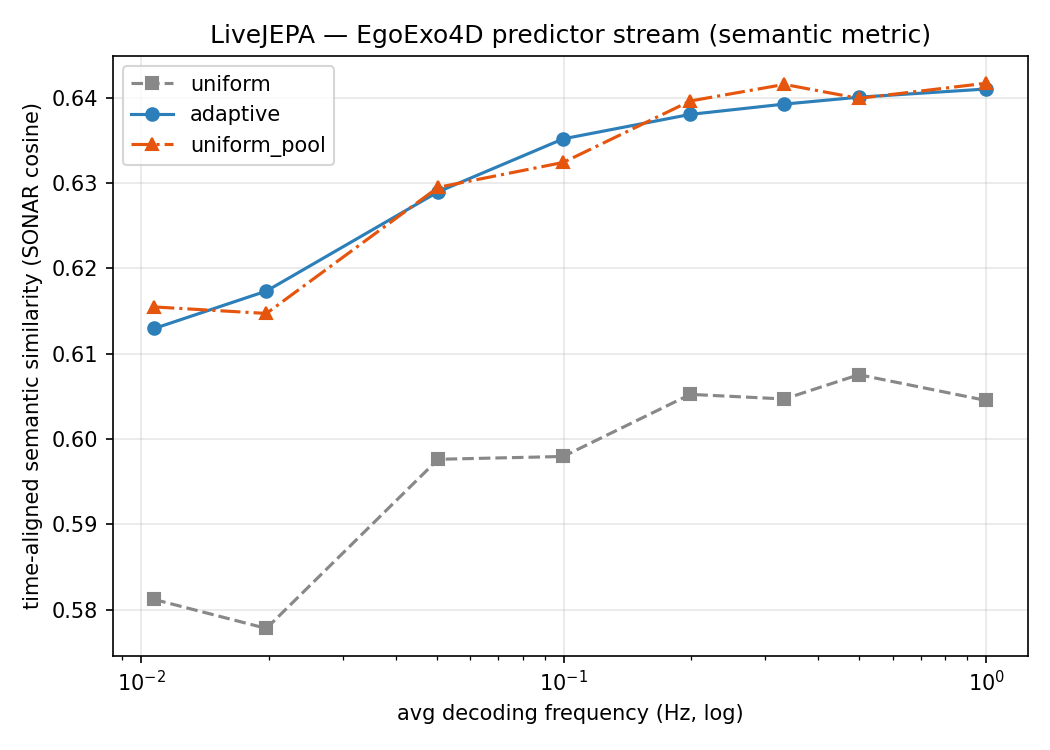
\includegraphics[width=0.48\textwidth]{figures/results_egoexo_predictor_40_indomain_semantic_nopool_pooled.png}
\caption{Controls on the semantic metric, same takes. Left: with pooling,
uniform+pool sits just above adaptive at every budget. Right: with mean-pooling
disabled but the pre-smoothing still applied, adaptive's flat lead over plain
uniform vanishes against uniform points given the same smoothing --- the margin
once read as temporal selection was the smoothing.}
\label{fig:controls}
\end{figure*}

\begin{figure*}[t]
\centering
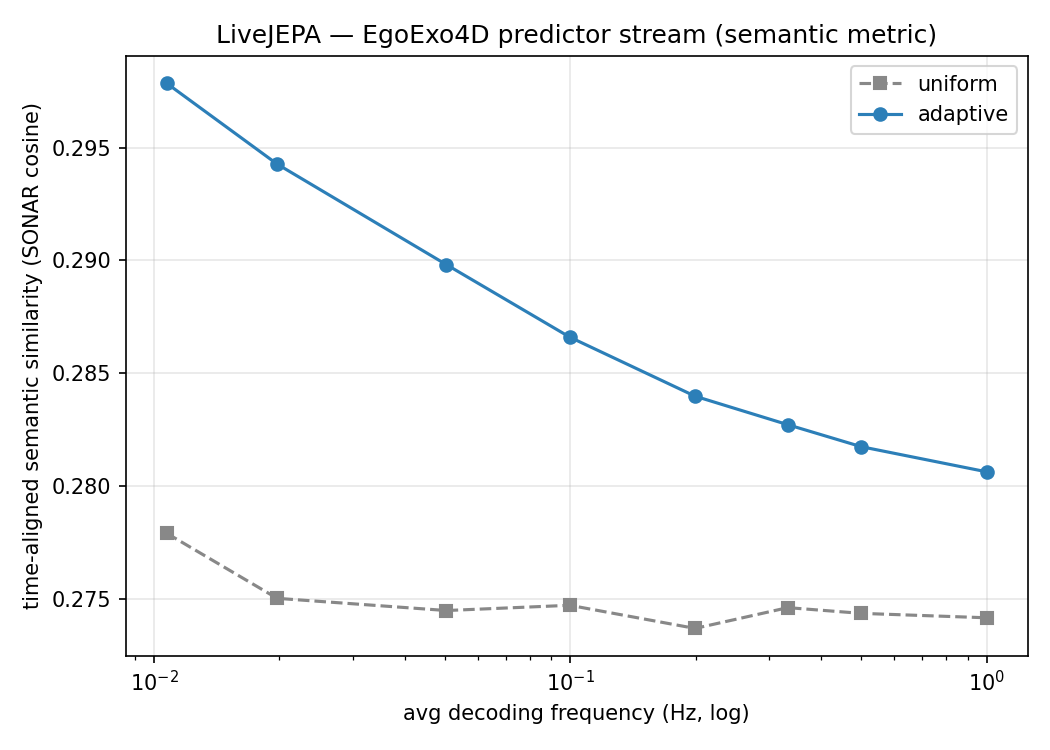
\includegraphics[width=0.48\textwidth]{figures/results_egoexo_predictor_40_semantic.png}
\hfill
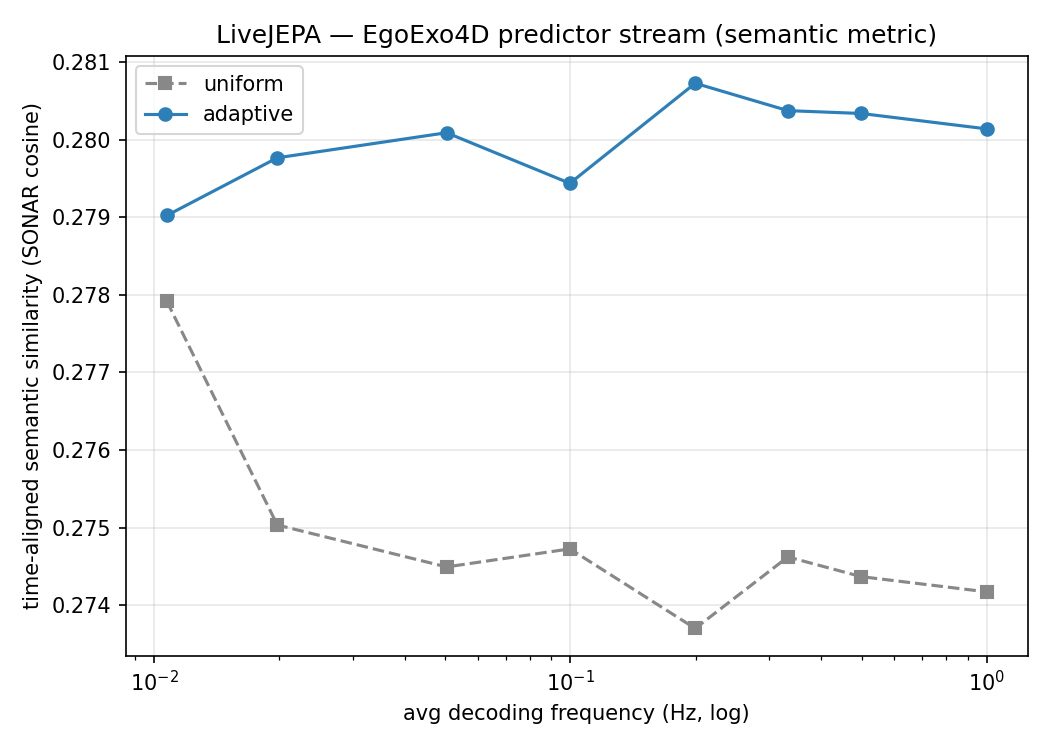
\includegraphics[width=0.48\textwidth]{figures/results_egoexo_predictor_40_semantic_nopool.png}
\caption{The rejected result, retained because the original controls were defined
against it. An out-of-domain predictor appeared to win 8/8 on the semantic metric
(left), but with pooling disabled the advantage collapses (right): that effect was
denoising, not selection. The in-domain run's apparent survival of the same check
rested on smoothing applied to adaptive alone.}
\label{fig:rejected}
\end{figure*}

\emph{Is it the takes rather than the stream?} The negative of
Section~\ref{sec:boundary} was measured on 218 takes and the predicted-stream
result on 40 of them, so we recomputed the ground-truth stream on exactly those 40
(Table~\ref{tab:sametakes}). Uniform still wins 7 of 8 budgets there --- adaptive
edges it only at 0.20~Hz --- against adaptive beating plain uniform at 7 of 8 on
the predicted stream. The reversal belongs to the stream, not to the take sample;
what the predicted stream rewards is averaging (Table~\ref{tab:headline}).

\begin{table}[t]
\caption{Same 40 takes, two streams. Ground-truth annotations favour uniform; on
the predicted stream adaptive beats plain uniform, a reversal that
Table~\ref{tab:headline} attributes to averaging.}
\label{tab:sametakes}
\centering
\footnotesize
\setlength{\tabcolsep}{4pt}
\begin{tabular}{rcccc}
\toprule
& \multicolumn{2}{c}{ground-truth stream} & \multicolumn{2}{c}{predicted stream} \\
\cmidrule(lr){2-3}\cmidrule(lr){4-5}
Hz & uniform & adaptive & uniform & adaptive \\
\midrule
1.00 & \best{4.51} & 3.68 & 0.296 & \best{0.330} \\
0.50 & \best{3.49} & 3.23 & 0.310 & \best{0.348} \\
0.35 & \best{2.95} & 2.85 & 0.299 & \best{0.340} \\
0.20 & 2.35 & \best{2.38} & 0.287 & \best{0.333} \\
0.10 & \best{1.84} & 1.71 & 0.282 & \best{0.331} \\
0.05 & \best{1.52} & 1.30 & 0.278 & \best{0.338} \\
0.02 & \best{1.16} & 0.99 & 0.249 & \best{0.312} \\
0.01 & \best{1.04} & 0.88 & \best{0.305} & 0.302 \\
\bottomrule
\end{tabular}
\end{table}

\subsection{Significance and headroom}
\label{sec:rigor}
\emph{Are the margins real across only 40 videos?} Tables~\ref{tab:sig}
and~\ref{tab:sigpool} and Fig.~\ref{fig:rigor} report the paired bootstrap against
each baseline. Against
plain uniform the semantic margin is significant at all eight budgets, with 40 of
40 takes favouring adaptive at seven of them, and per-take CIDEr favours adaptive
at seven budgets, significantly at all seven; at the degenerate 0.011~Hz point the
difference is null. Against uniform+pool the semantic metric reverses ---
uniform+pool is significantly ahead at all eight budgets --- and per-take CIDEr is
tied at six, with adaptive significantly ahead at 0.05~Hz ($+0.014$) and
significantly behind at 0.35~Hz ($-0.011$). One significant cell each way among
eight is what no consistent effect looks like. CIDEr has visibly lower power than
the semantic metric, because n-gram overlap over roughly a hundred events is
high-variance where cosine similarity is smooth.

\begin{table}[t]
\caption{Paired bootstrap against plain uniform, 40 held-out takes, 5{,}000
resamples. $\Delta$ is adaptive $-$ uniform; $n^{+}$ is takes favouring adaptive.
Bold marks intervals clear of zero.}
\label{tab:sig}
\centering
\footnotesize
\setlength{\tabcolsep}{3pt}
\begin{tabular}{rccrccr}
\toprule
& \multicolumn{3}{c}{semantic} & \multicolumn{3}{c}{per-take CIDEr} \\
\cmidrule(lr){2-4}\cmidrule(lr){5-7}
Hz & $\Delta$ & 95\% CI & $n^{+}$ & $\Delta$ & 95\% CI & $n^{+}$ \\
\midrule
1.00 & \textbf{+.040} & [+.035,+.044] & 40 & \textbf{+.019} & [+.007,+.032] & 26 \\
0.50 & \textbf{+.042} & [+.036,+.048] & 40 & \textbf{+.021} & [+.009,+.033] & 26 \\
0.35 & \textbf{+.048} & [+.042,+.054] & 40 & \textbf{+.025} & [+.011,+.041] & 28 \\
0.20 & \textbf{+.052} & [+.046,+.059] & 40 & \textbf{+.026} & [+.006,+.049] & 23 \\
0.10 & \textbf{+.067} & [+.058,+.076] & 40 & \textbf{+.030} & [+.011,+.050] & 28 \\
0.05 & \textbf{+.078} & [+.067,+.089] & 39 & \textbf{+.028} & [+.007,+.050] & 27 \\
0.02 & \textbf{+.106} & [+.090,+.121] & 40 & \textbf{+.037} & [+.009,+.068] & 27 \\
0.01 & \textbf{+.106} & [+.086,+.126] & 40 & $-.002$ & [$-$.037,+.031] & 19 \\
\bottomrule
\end{tabular}
\end{table}

\begin{table}[t]
\caption{Paired bootstrap against uniform+pool, the pooling-matched baseline.
$\Delta$ is adaptive $-$ uniform+pool; $n^{+}$ is takes favouring adaptive. Bold
marks intervals clear of zero.}
\label{tab:sigpool}
\centering
\footnotesize
\setlength{\tabcolsep}{3pt}
\begin{tabular}{rccrccr}
\toprule
& \multicolumn{3}{c}{semantic} & \multicolumn{3}{c}{per-take CIDEr} \\
\cmidrule(lr){2-4}\cmidrule(lr){5-7}
Hz & $\Delta$ & 95\% CI & $n^{+}$ & $\Delta$ & 95\% CI & $n^{+}$ \\
\midrule
1.00 & \textbf{$-$.001} & [$-$.002,$-$.001] & 12 & $-$.006 & [$-$.016,+.003] & 21 \\
0.50 & \textbf{$-$.002} & [$-$.003,$-$.001] & 12 & $-$.000 & [$-$.009,+.007] & 24 \\
0.35 & \textbf{$-$.003} & [$-$.004,$-$.002] & 7 & \textbf{$-$.011} & [$-$.020,$-$.002] & 11 \\
0.20 & \textbf{$-$.004} & [$-$.006,$-$.003] & 3 & $-$.003 & [$-$.012,+.008] & 15 \\
0.10 & \textbf{$-$.007} & [$-$.009,$-$.005] & 2 & $-$.006 & [$-$.018,+.005] & 21 \\
0.05 & \textbf{$-$.007} & [$-$.009,$-$.005] & 5 & \textbf{+.014} & [+.006,+.023] & 29 \\
0.02 & \textbf{$-$.010} & [$-$.016,$-$.005] & 5 & $-$.003 & [$-$.017,+.010] & 13 \\
0.01 & \textbf{$-$.011} & [$-$.018,$-$.005] & 1 & $-$.008 & [$-$.021,+.006] & 9 \\
\bottomrule
\end{tabular}
\end{table}

\begin{figure}[t]
\centering
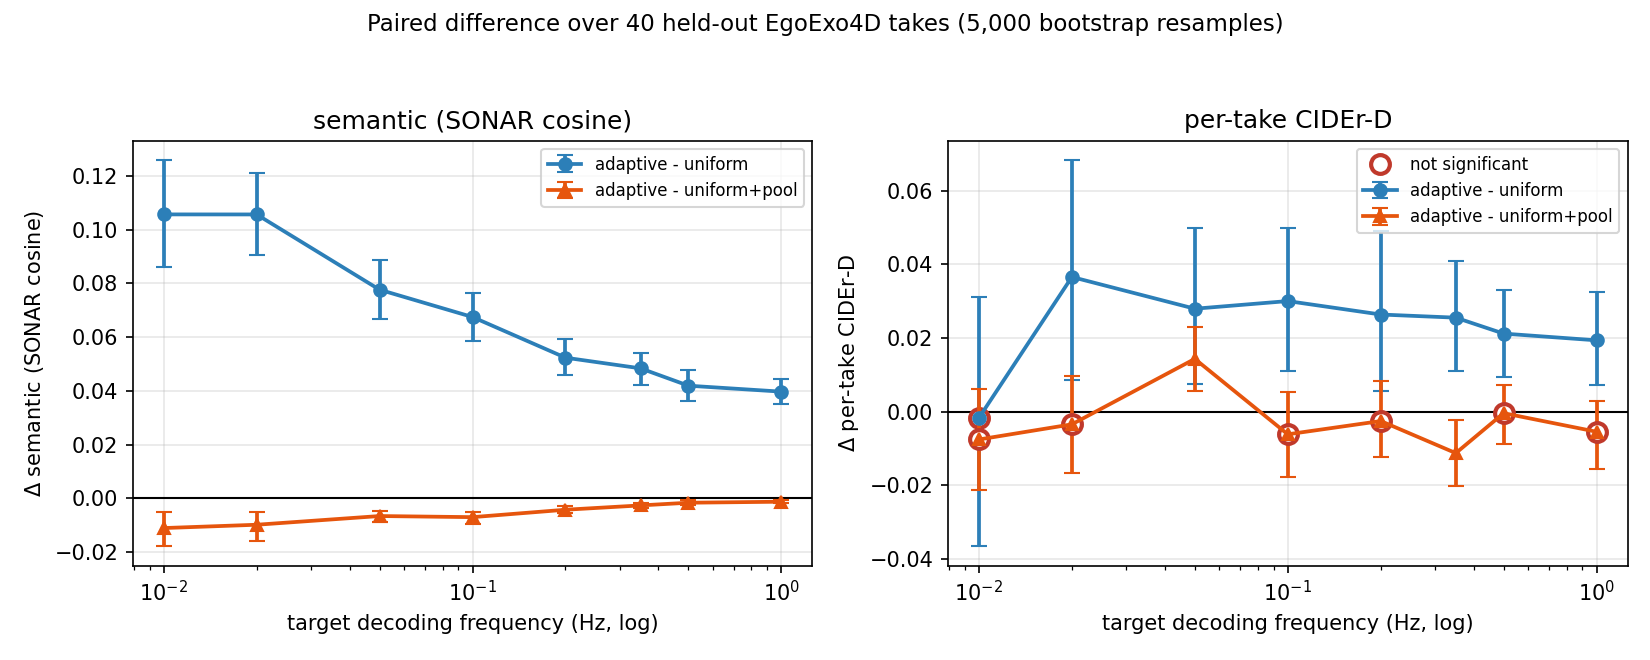
\includegraphics[width=\columnwidth]{figures/results_egoexo_rigor.png}
\caption{Paired per-take difference between adaptive and each baseline, with 95\%
intervals. Against single-point uniform adaptive is ahead on both metrics; against
uniform+pool the semantic difference is negative at every budget and the CIDEr
difference straddles zero. Non-significant cells are circled.}
\label{fig:rigor}
\end{figure}

\emph{What can the ceiling show?} For each annotation, the \emph{best-window
ceiling} takes the maximum of
$\cos(\mathrm{mean}(S[a{:}b]), \mathrm{SONAR}(y))$ over all contiguous ranges
$[a{:}b]$. Every schedule here decodes either a stream point or a pooled
contiguous span, so this upper-bounds every row of Table~\ref{tab:ceiling} and
Fig.~\ref{fig:ceiling};
computing it on the smoothed stream as well, and taking the per-annotation maximum
over both, moves the bound by 0.0001, so the figure in the table stands.

Three findings follow. First, \emph{pooling beats decoding more}: single-point
decoding is flat in rate, and every pooled schedule exceeds decode-everything at a
fraction of its cost, so on a noisy predicted stream averaging before decoding is
not a quality/compute trade-off but a strict improvement; the $+0.018$ gap between
the best-window and best-frame ceilings confirms that a pooled span carries signal
no single timestep does. Second, \emph{where the boundaries fall barely matters}:
Ward boundaries (0.6725), the annotators' own boundaries (0.6684) and fixed blocks
(0.6791) land within 0.011 of one another. Third, \emph{the bound cannot rank
triggers here}: a schedule with no trigger at all --- one mean per take --- reaches
90.0\% of it, above every adaptive budget, because a take-level summary sits close
to most of a repetitive take's captions. Adaptive's 87.1\% therefore does not show
a near-exhausted trigger, as an earlier version of this analysis concluded; the
metric rewards averaging in itself, and can compare schedules only at matched
pooling.

\begin{table}[t]
\caption{Headroom on the semantic metric (40 takes, 95\% bootstrap intervals), as
a percentage of the best-window ceiling.}
\label{tab:ceiling}
\centering
\footnotesize
\setlength{\tabcolsep}{4pt}
\begin{tabular}{lcc}
\toprule
reference & score (95\% CI) & \% ceiling \\
\midrule
uniform @0.05~Hz & 0.5949 [.5740, .6167] & 77.1 \\
dense (every timestep) & 0.6037 [.5854, .6243] & 78.2 \\
GT-boundary trigger & 0.6684 [.6522, .6851] & 86.6 \\
adaptive @0.05~Hz & 0.6725 [.6560, .6898] & 87.1 \\
uniform+pool @0.05~Hz & 0.6791 [.6626, .6963] & 88.0 \\
one decode per take & 0.6950 [.6791, .7117] & 90.0 \\
best-frame ceiling & 0.7541 [.7396, .7692] & 97.7 \\
\textbf{best-window ceiling} & \textbf{0.7720} [.7577, .7867] & 100 \\
\bottomrule
\end{tabular}
\end{table}

\begin{figure}[t]
\centering
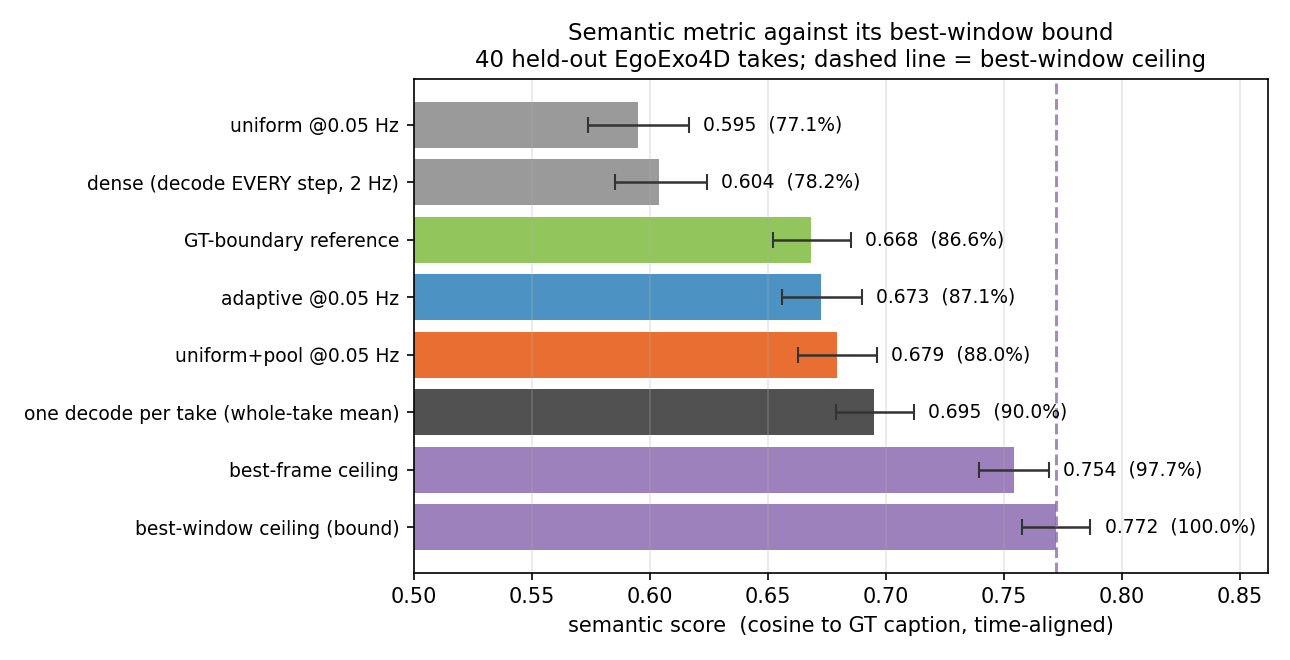
\includegraphics[width=\columnwidth]{figures/results_egoexo_ceiling.png}
\caption{The semantic metric against its best-window bound. Every pooled schedule
beats decoding every frame, whichever boundaries it uses, and a single whole-take
mean, with no timing at all, scores highest of all --- so the bound measures how
well pooled summaries match captions, not how good a trigger is.}
\label{fig:ceiling}
\end{figure}

A provenance note belongs with this analysis. Our first boundary oracle scored
\emph{below} uniform, which is impossible for an upper bound. It was a code fault:
the ground-truth stream is timestamped from $t=0$ while the predicted stream
carries window-centre times beginning $\approx$3.75~s in, so index-based mapping
misaligned every decode by about four seconds. After the fix the oracle still did
not exceed adaptive, and the right conclusion was that the label ``oracle'' was
wrong, not the number. An upper bound that loses to the method it bounds is a bug;
one that merely ties is a finding.

\section{Discussion}

\subsection{Placement on clean streams, averaging on predicted ones}
On clean ground-truth streams, where decodes are placed decides quality. Adaptive
placement beats uniform across the mid-band on COIN steps and EgoExo keysteps, and
on the raw atomic-annotation stream, where an event lands every two seconds, it
loses at every budget: the value of placing decodes adaptively tracks the
redundancy of the stream it reads. On a predicted stream, averaging decides
quality. Against single-point uniform, adaptive wins 7 of 8 budgets over the same
40 atomic takes where the annotation stream favours uniform, but what it brings to
the noisy predicted stream is pooling: given the same pooling, uniform decoding
matches adaptive on CIDEr and beats it on the semantic metric. VL-JEPA reports both
that pooling helps both schedules and that adaptive selection Pareto-dominates
uniform; in our reconstruction the first replicates and the second does not. On
COIN's predicted stream, where adaptive was compared with \emph{plain} uniform and
still lost the mid-band because 0.2~Hz is COIN's intrinsic step cadence, the same
reading applies with more force. For a practitioner the rule is operational: on a
clean, sparse stream, place decodes on change; on a predicted stream, pool before
decoding, and a fixed grid will do.

\subsection{A predictor problem, not a mechanism problem}
Separating the two axes is the most transferable result here. Caption correctness
--- vocabulary, object detail, register --- is a property of the predictor and its
training data; the selective policy decides \emph{when} to speak, not \emph{what}
to say. The evidence is direct: replacing a COIN-trained predictor with an
in-domain one raised CIDEr $25\times$ on the same takes, the COIN scaling curve had
not flattened at 9$\times$ the data, and on the predicted stream the choice between
adaptive and fixed-interval spans made no consistent difference. Effort spent
tuning thresholds was, in retrospect, misdirected: every such attempt in this work
returned negative.

\subsection{Methodological note}
Four times a positive result failed its own controls. An out-of-domain semantic
win proved to be denoising rather than selection; a ``noisy labels'' explanation
for the Action100M negative was contradicted by measurement and replaced by the
entropy account; an upper bound that lost to the method it bounded turned out to
be a time-alignment bug; and the headline of an earlier version of this paper ---
adaptive winning 7 of 8 budgets on the predicted stream at $\approx 9.9\times$
fewer decodes --- did not survive a uniform baseline given the pooling the original
paper gives it, because the control meant to rule averaging out had left the
pre-smoothing on one side only. A control is only as good as the match between its
two arms: every difference between them other than the hypothesis is a confound
until it is removed.

\section{Limitations}
The COIN predicted-stream evaluation rests on 7 held-out videos, since extraction
deleted source video after caching; its low-frequency tail is noise. The
predicted-stream comparison uses 40 takes rather than the full 218-take pool, at
about 23 minutes of encoding per take; more takes would tighten the ties between
adaptive and uniform+pool. The evaluation takes are disjoint from training by take
but not by person or session: all 40 share a participant with training takes and
39 share a recording session, so absolute quality partly reflects that
familiarity, although all schedules consume the same stream. A participant-disjoint
retrain needs no new extraction --- filtering the existing cache keeps 483 takes
and 8{,}822 pairs, 76\% of the data --- and is the most useful next control. The
non-replication is specific to our reconstruction: our predictor (29.9M
parameters, in-domain) and embedding space differ from VL-JEPA's (490M parameters,
trained on Action100M), and a predictor with crisper semantic structure might
restore a placement advantage at matched pooling; the original paper also does not
state the window over which its uniform baseline pools, and ours --- one decode
interval around each point --- is one reasonable choice. Results from the
data-scaling study onward use a single pre-smoothing setting that was never tuned
on EgoExo. The semantic metric --- ours, not the paper's --- rewards averaging in
itself, so it compares schedules only at matched pooling, and the benchmark is
weakly sensitive to timing: one caption per take scores about as well as uniform
decoding at 0.2~Hz. CIDEr has low statistical power at these scales. Finally, the
pipeline is not real-time on the test hardware, at $\approx$11~s per window on a
T1000; deployment would need a faster encoder or a coarser working rate.

\section{Future Work}
The evidence orders the next steps. First, predictor capacity and in-domain data,
the lever for caption quality; the entropy analysis predicts the route is one to
two orders of magnitude more open-vocabulary data rather than a different mixing
strategy. Second, an evaluation protocol that rewards timing --- for example,
scoring only annotations that differ from their take's typical content, or
reporting every schedule against the one-caption-per-take reference --- so that
placement can show whatever value it has. Third, the participant-disjoint retrain,
which would close the one methodological gap in the absolute numbers at no data
cost, and scaling the predicted-stream comparison from 40 to 218 takes. Fourth, a
hybrid policy --- a pooled uniform floor plus extra decodes on detected change ---
as the most plausible way for placement to add to pooling. Fifth, pairing the
trigger with a strong pretrained captioner, since the trigger is decoder-agnostic
and such a captioner would supply the open-domain vocabulary this reconstruction
lacks.

\section{Conclusion}
We reconstructed VL-JEPA's selective-decoding mechanism from released components,
corrected its causal realisation, and stress-tested it against its own claims.
Selective decoding beats uniform across the mid-band on temporally redundant
streams and loses at every budget on raw dense annotations. On a predicted stream
over the same annotations it beats single-point uniform decoding at 7 of 8 budgets,
but the gain is averaging: given the same pooling, which the original paper gives
both schedules, uniform decoding matches adaptive --- tied at six of eight budgets
with one significant win each way --- and reaches a higher best score. In our
reconstruction the paper's adaptive-over-uniform result therefore holds on clean,
redundant streams but does not replicate like for like on a predicted one, where
what pays is averaging the predictor's noise before decoding, under any schedule;
and a benchmark on which one caption per video scores like a 0.2~Hz schedule
leaves little room for any trigger to show its worth. What limits caption quality
is the predictor: a scaling curve that has not flattened, a $25\times$ gain from
in-domain data, and a question of target-vocabulary entropy rather than of domain
match.

\bibliographystyle{IEEEtran}
\bibliography{references}

\end{document}
